\documentclass{resume}

\name{Jiangkun QIU}
\address{\faPhone~+86 158 6659 6952 \faEnvelope~\href{mailto://qjk2001@gmail.com}{qjk2001@gmail.com} \faGithub~\href{https://github.com/qiujiangkun/}{GitHub: qiujiangkun} \faWeixin~rocon2001 ~~~~~}
\address{Target: Backend Development}

\begin{document}

\begin{tikzpicture}[remember picture, overlay] 
    \node[anchor = north east] at ($(current page.north east)+(-1.3cm,-1.2cm)$) {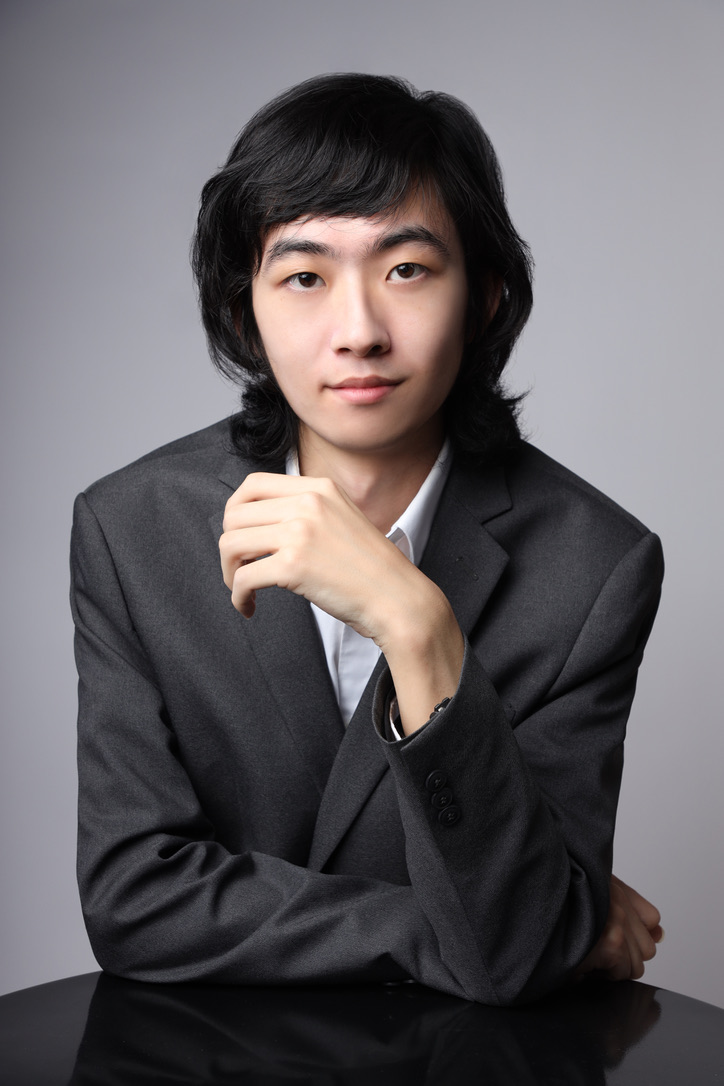
\includegraphics[height=2.5cm]{avatar.jpg}};
  \end{tikzpicture}

\begin{rSection}{\faCogs~Skill Set}
    \begin{itemize}
        \itemsep -0.5em
        \item Programming experience for 9 years since 10
        \item Trained intensively in algorithms and data structures and get awards in Informatics
        \item Familiar with C, C++, Java, Python, Rust and Scala
        \item Basic experience in JavaScript, HTML, PHP, C\#, SQL, Bash
        \item Hands-on experience in Linux and git on daily basis for years
        \item Comprehend operating system, network, machine learning, deep learning, Kafka, K8S, Netty, Disruptor, concurrent programming, JVM optimization
    \end{itemize}
    
\end{rSection}

\begin{rSection}{\faGraduationCap~Education}
    % \begin{rSubsection}{Secondary Education}{}{}{}
    %     \item Weifang New Epoch School, Shandong Province, China \hfill Sep 2017-Jun 2020
    %     \item Weifang Guangwen Middle School, Shandong Province, China \hfill Sep 2014-Jun 2017
    % \end{rSubsection}
    Hong Kong University of Science and Technology, China \hfill Sep 2020-Now \\ Integrated System and Design(Programming) major
\end{rSection}

\begin{rSection}{\faUsers~Working Experienes}
    \begin{rExperience}{Internship Server Arch}{Beijing ByteDance Technology Co., Ltd.}{2022.04-2022.09}
        \begin{itemize}
            \itemsep -0.5em \vspace{-0.5em}
            \item According to company's demand, write a universal and customizable API Linter, supporting both ProtoBuf and Thrift, running as a CLI tool and an gitlab CI task
            \item Maintain and improve on DevFlow, letting it support more products. It's a platform that integrates a fluent online editor, peer review for API changes, linting, compatibility check, code generation
            \item Maintain and improve on Overpass, a widely used platform that collects RPC definition files and generate RPC client for other go projects
        \end{itemize}
    \end{rExperience}
    \begin{rExperience}{Full-time Backend Dev}{ERX Inc, Thailand}{2022.03-今}
        \textbf{项目背景}:
        Rewrite ERX.io, the only licensed "digital asset" exchange in Thailand\\
        \textbf{项目内容}
        \begin{itemize}
            \itemsep -0.5em \vspace{-0.5em}
            \item Rewrite a Tezos smart contract from the obscure Haskell Morley to clear SmartPy code
            \item Build the exchange from scratch, involved in regulatory compilance, architecture, database design, API design and development, matching engine MVP development
            \item Research on cryptography and HSM, implement wallets for crypto on-chain transaction signing
        \end{itemize}
    \end{rExperience}
    \begin{rExperience}{Full-time Backend Dev}{Infinity Force Inc, Singapore}{2022.02-2022.04}
        \textbf{项目背景}:
        Build a account rental platform for the game Axie Infinity\\
        \textbf{项目内容}
        \begin{itemize}
            \itemsep -0.5em \vspace{-0.5em}
            \item Implement Infinity Force Token in Solidity
            \item Optimize the original Python+Postgres backend stack with Rust.Optimize workflow with Code Generation
            \item Exploit the private APIs of the game to manage NFT assets with web3 package on the platform
        \end{itemize}
    \end{rExperience}
    \begin{rExperience}{Backend Internship}{Shanghai Rangchuan Information Technology Co., Ltd.}{Dec 2020-Now}
        \begin{itemize}
            \itemsep -0.5em \vspace{-0.5em}
            \item Distributed Rate Limiter: Implemented  a modified version of the Sliding Log algorithm With Akka and Redis, to restrict service usage for each user and API. This solved the incapacity that distributed nodes cannot constrict use rate within a small number after load balancing with Ingress in K8S
            \item WeChat Work Third Party Application:Developed a WeChat Enterprise third-party App prototype with Python to boost intelligent hiring
            \item Slow Speed Refresh Service:Read changelog from PostgreSQL,clense changelog for each tenant company and write to different Kafka topics according to configuration;Implement a Slow Speed Refresh Queue and its Web Dashboard for internal use with restricted SQL injection       
        \end{itemize}
    \end{rExperience}
    \begin{rExperience}{Part-time Job}{A quantitative trading company of digital currencies}{Jul 2020-Now}
        \begin{itemize}
            \itemsep -0.5em \vspace{-0.5em}
            \item Developed, from scratch in Rust, a set of libraries to collect and process data from dozens of trading platforms. Utilize cache line, lockless ring buffer, etc, to implement a 1:1 thread model and boost performance. Implemented a UDP proxy to work around AWS whitelist.
            \item Set up a web-based monitoring system with InfluxDB ReactJS, Flask and Plotly Dash
            \item Built a distributed backtesting system. Collect data from trading platforms to Kafka, and automatically deploy backtesting tasks to AWS autoscaling groups with ansible, then collect backtesting data to PostgreSQL and TimescaleDB.
            \item Implemented a json deserialization libray with Rust procedual macros and outperform the classic Serde libray by one time.
        \end{itemize}
    \end{rExperience}

\end{rSection}

\begin{rSection}{\faUsers~Projects}
    % TODO add a Java backend project
    \begin{rProject}{School Research}{The SHLL Programming language}{2022.01-Now}
        \textbf{Reasons}: SHLL is a programming language for researching high-level compiler optimization, hoping facilitate development of High-Frequency Trading software. SHLL borrows some ideas from a similar school project, which is badly written, but has more engineering, aesthetic and agronomical considerations\\
        \textbf{Development}: Build a user-friendly, beautiful language, which utilizing analyzing code, specialization and inlining to eliminate abstraction cost, achieving the true zero-cost abstraction. Use scala 3 as the front-end language, to ensure expressiveness of the language
    \end{rProject}
    \begin{rProject}{Personal Project}{Unidef}{2021.07-Now}
        \textbf{项目概述}: Unidef a tool for type to type conversion across languages, for code generation and transpilation. Written originally in Python but written in Scala\\
        \textbf{项目开发}: maintain a set of ASts, which try to keep all nuance of source languages and be language netural and consistent. It supports JSON, Json Schema, FIX, primary programming languages. It's also the base for SHLL
    \end{rProject}
    % \begin{rProject}{Collaborated Project}{WP-Reliable MD}{Sep 2018-Aug 2019}
    %     \textbf{Reasons}: Since the Markdown plugin I was using ceased to develop, my friends and I managed to introduce the Markdown Tui-Editor to WordPress Plugin Marketplace\\
    %     \textbf{Duties}
    %     \begin{itemize}
    %         \itemsep -0.5em \vspace{-0.5em}
    %         \item Project Management: As the team leader, I proposed the overall architecture and technical choice. I was also in charge of early development
    %         \item Project Development: Redesign the GUI for Tui-Editor and replaced the original editor of WordPress. Adopted a RESTful API to render MarkDown text to work around the incapacity of rendering LaTeX math equations in places other than plaintext. Use a non-intrusive approach to avoid data lose and inconsistency when the plugin is down.
    %     \end{itemize}
    % \end{rProject}

% \begin{rSubsection}{\href{https://github.com/qiujiangkun/Escape}{Escape Game}}{Feb 2020}{Personal Project}{}
%     \item A 2D bird-view shooting game designed as an AI playground.
%     \item Adopted C++, Lua, ECS, Serialization, Box2D, Meta Template Programming.
%     \item 5k code in total
% \end{rSubsection}
% \begin{rSubsection}{\href{https://github.com/qiujiangkun/EnglishPassageReader}{English Passage Reader}}{Apr 2019}{Personal Project}{}
%     \item A web application aimed to help non-native English speakers read English.
%     \item Applied Python Flask, JavaScript and HTML
% \end{rSubsection}

% \begin{rSubsection}{\href{https://github.com/qiujiangkun/ZhuoxinSocialWebsite}{Zhuoxin Social Platform}} {Oct 2018}{Personal Project}{}

% \item Developed a website like PenPal World and Facebook, from scratch, with full functionality.

% \item Applied PHP, HTML, JavaScript, MySQL, and Semantic UI and concepts of network security and abstraction.

% \end{rSubsection}

\end{rSection}

\begin{rSection}{\faAward~Awards and Certifications}
    \begin{itemize}
        \itemsep -0.5em

        % \item Third Prize in the Interdisciplinary Cup in Information Technology Applications \\ in Shandong Province \hfill Dec 2018
        \item China Computer Federation Certified Student Member \hfill Jul 2019-Now

        \item First Prize in the High School Group of National Informatics Olympiad in Provinces \hfill Nov 2017, Nov 2018
        \item Gold Award of RoboCom2018 Global Championship(Robot Competition) \hfill Jul 2018
        % \item First Prize in Personal Skills of RoboCom2018 Global Championship \hfill Jul 2018
        % \item Best Programmer Prize of RoboCom2018 Global Championship \hfill Jul 2018
        % \item Second Prize in Star of Outlook - English Talent Competition, CCTV \hfill Apr 2018
        \item Second Prize in 2017 Tsinghua University Dengfeng Cup Data Mining Competition \hfill Jul 2018
        % \item Second Prize in China Shandong Student Maker (CSSM) Competition \hfill May 2017
        \item National Computer Rank Examination Level 4, Network Engineer \hfill Nov 2016
        \item First Prize(6th) in the Middle School Group of National Informatics Olympiad in Provinces \hfill Oct 2016
        \item First Prize(1st) in national finals of 19th He Education Cup Computer Competition \hfill Jul 2016
        % \item 3rd in the Weifang Experimental and Practical Competition \hfill Jul 2015
        
        % \item Qualification Certify for National Youth Robotics Level Test, Second Class \hfill Oct 2018
        % \item National Computer Rank Examination Level 3, Network Technology \hfill May 2016
        % \item National Computer Rank Examination Level 2, C language \hfill Nov 2015
    \end{itemize}
\end{rSection}
\end{document}
